\section{Image cleaning in FACT}

\begin{frame}
    \centering
    {\Huge \textbf{Image cleaning in FACT}}
\end{frame}

\begin{frame}{Cleaning methods}
    \begin{columns}[T] % align columns
        \begin{column}{.48\textwidth}
            \textbf{Tailcuts cleaning}

            \begin{enumerate}
                \item "Two treshold procedure"
                \item Pixels above t1 are kept
                \item Signal pixels need at least n neighbors
                \item Neighboring pixels above t2 get added
            \end{enumerate}
        \end{column}
        \begin{column}{.48\textwidth}
            \textbf{FACT image cleaning}

            \begin{enumerate}
                \item Similar behaviour, but also uses information about the arrival times
                \item Pixels with a very different arrival time than their neighbours get removed
                %\item for now arrival times are integers in ctapipe -> limits search for optimal threshold
                \item Removes "lonely" pixels multiple times
                %\item one would assume less separated pixels
                \item Probably removes more pixels with the same thresholds
            \end{enumerate}
        \end{column}
    \end{columns}
\end{frame}

\begin{frame}{Sample MC event on a Flash Cam}
    \begin{figure}
        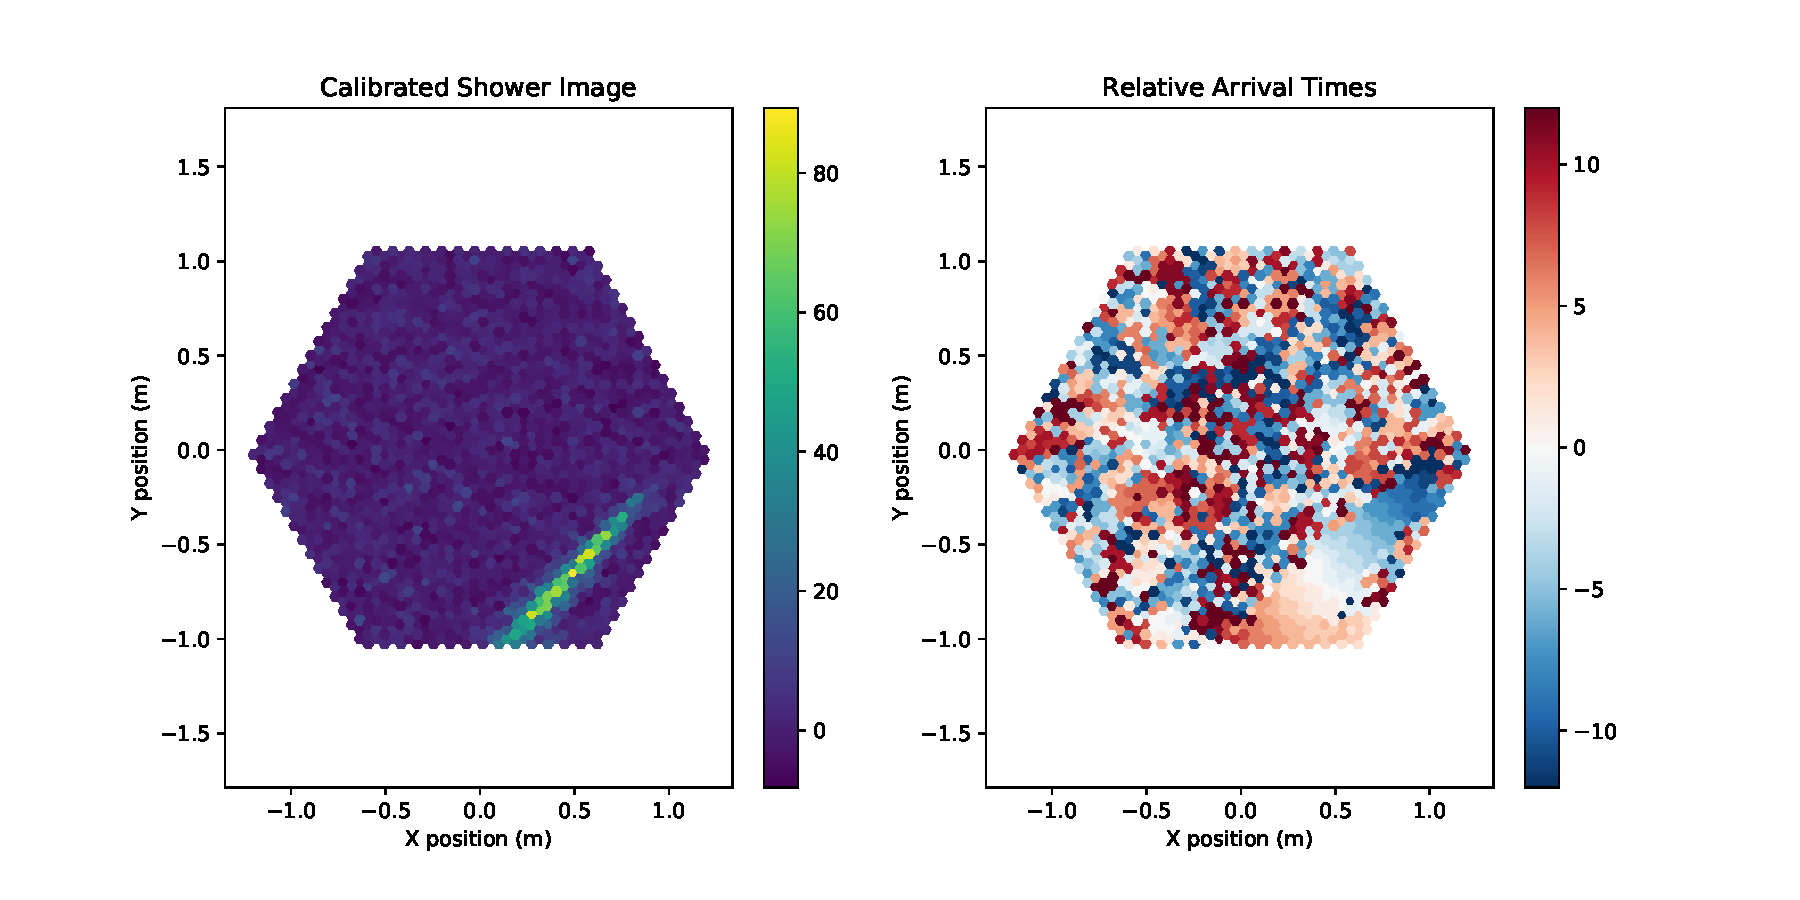
\includegraphics[width=\linewidth]{images/cleaning_plots/raw.pdf}
    \end{figure}
\end{frame}

% \begin{frame}{Cleaning: Tailcuts approach}
%     \begin{figure}
%         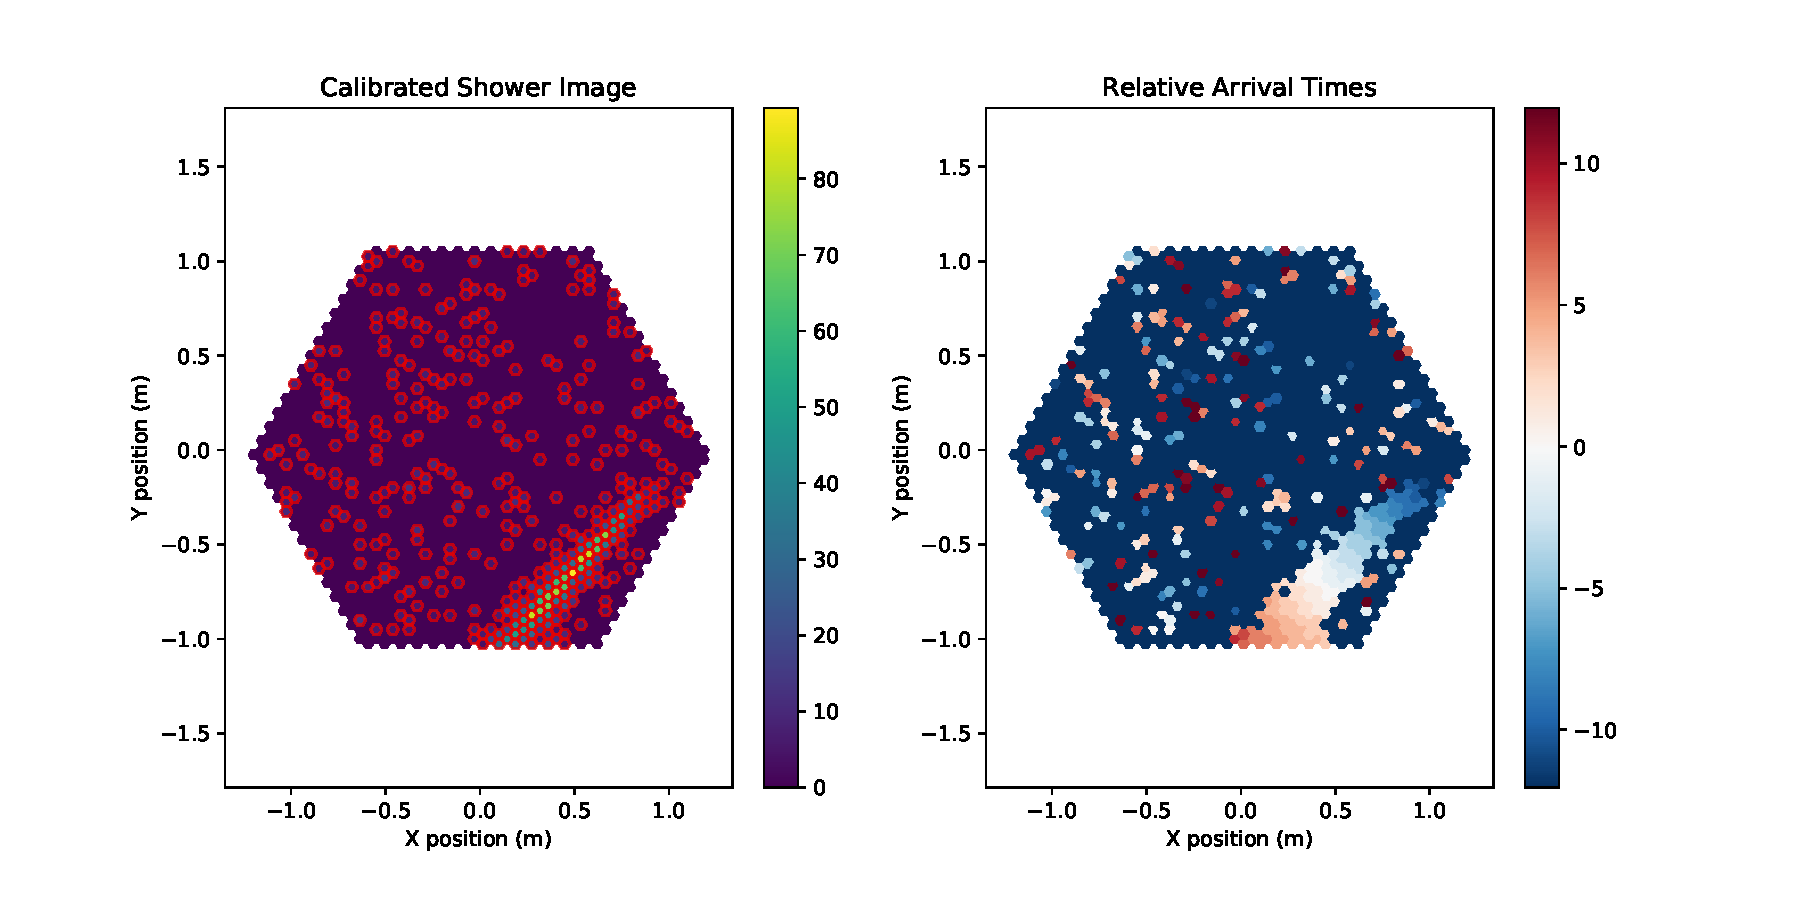
\includegraphics[width=\linewidth]{images/cleaning_plots/tail_1.pdf}
%     \end{figure}
% \end{frame}

% \begin{frame}{Cleaning: Tailcuts approach}
%     \begin{figure}
%         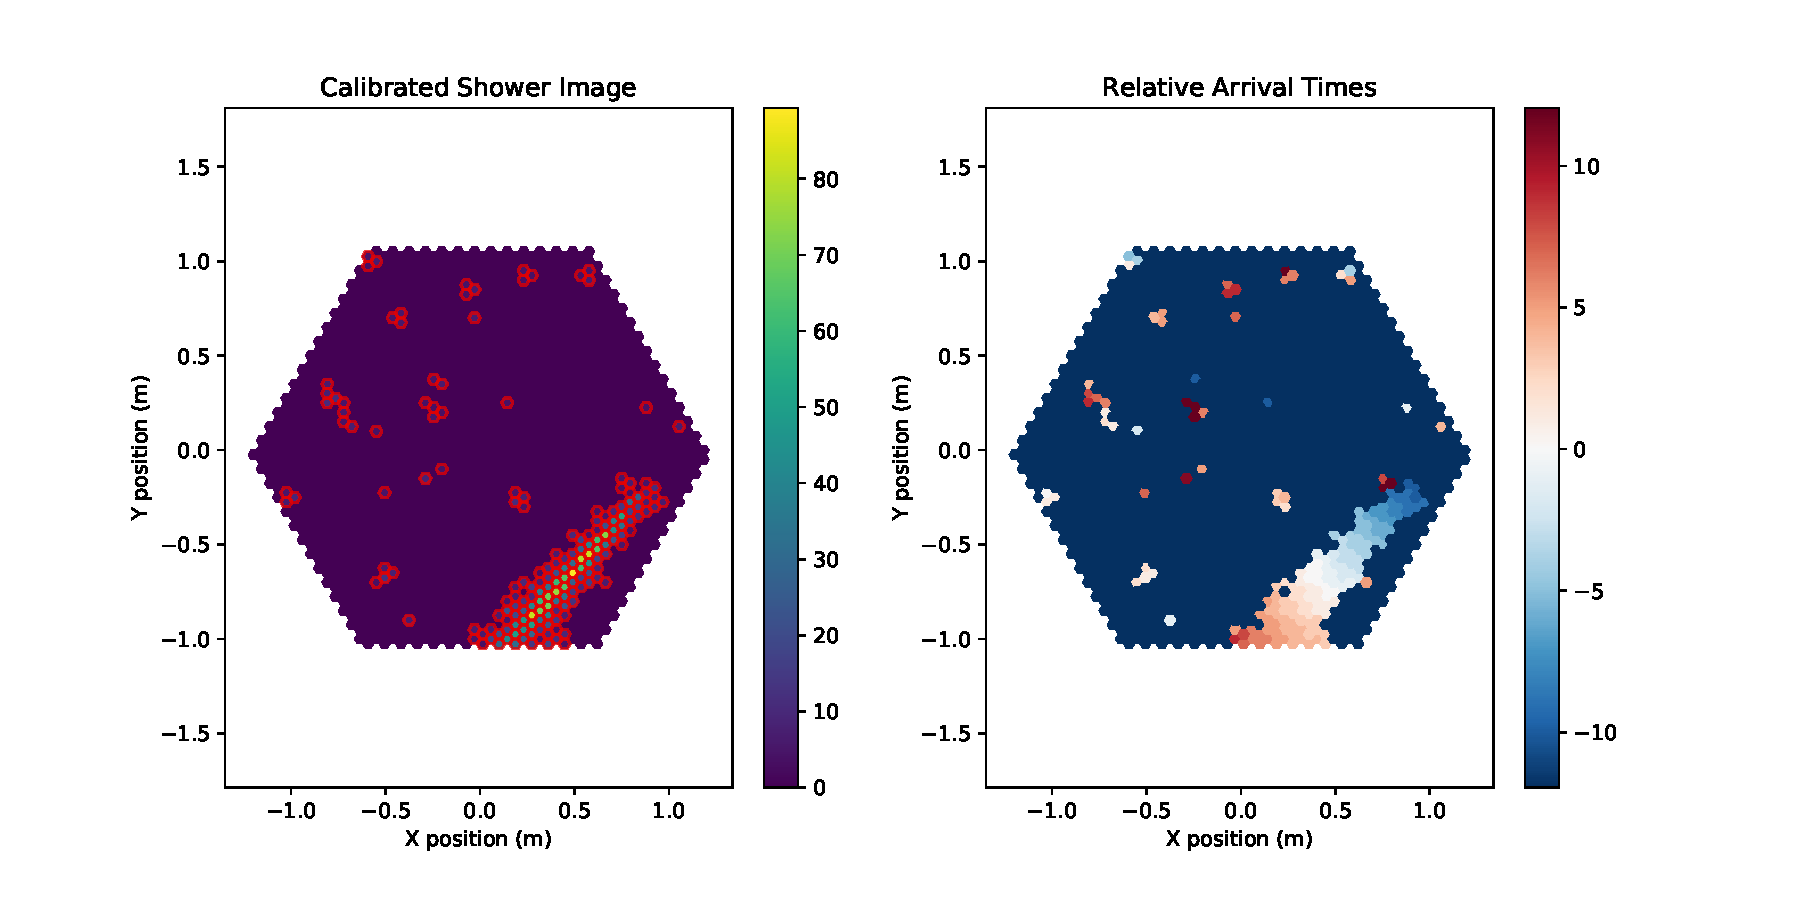
\includegraphics[width=\linewidth]{images/cleaning_plots/tail_2.pdf}
%     \end{figure}
% \end{frame}

% \begin{frame}{Cleaning: Tailcuts approach}
%     \begin{figure}
%         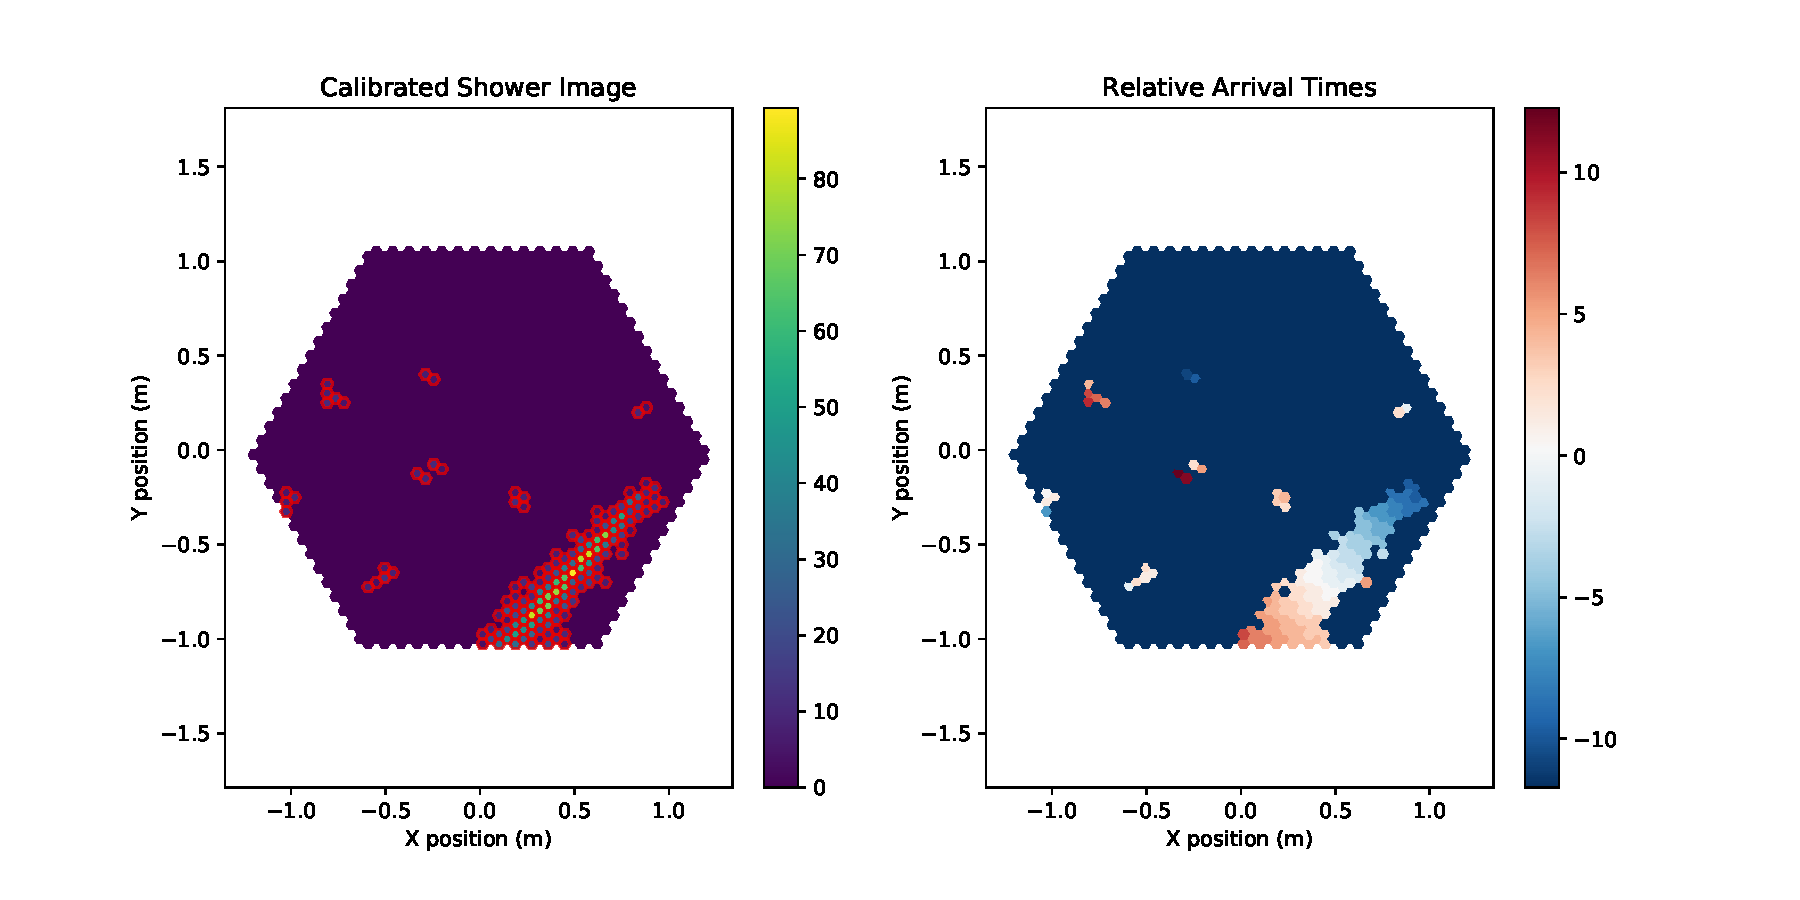
\includegraphics[width=\linewidth]{images/cleaning_plots/tail_3.pdf}
%     \end{figure}
% \end{frame}

% \begin{frame}{Cleaning: FACT approach}
%     \begin{figure}
%         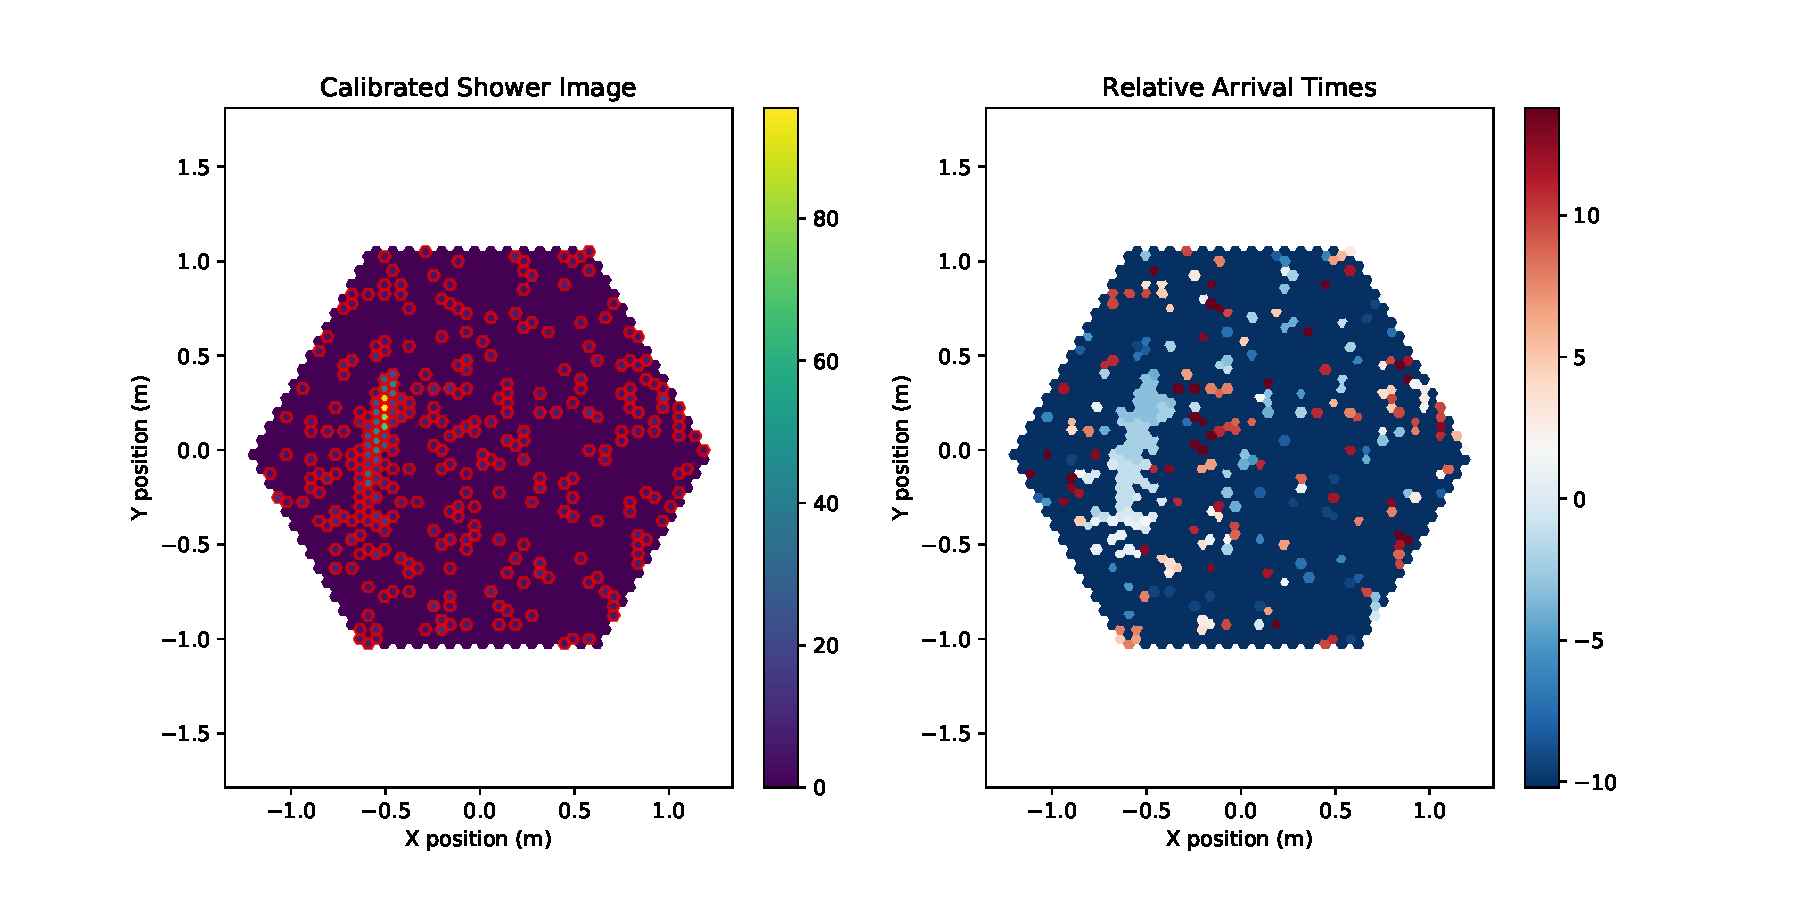
\includegraphics[width=\linewidth]{images/cleaning_plots/fact_1.pdf}
%     \end{figure}
% \end{frame}

% \begin{frame}{Cleaning: FACT approach}
%     \begin{figure}
%         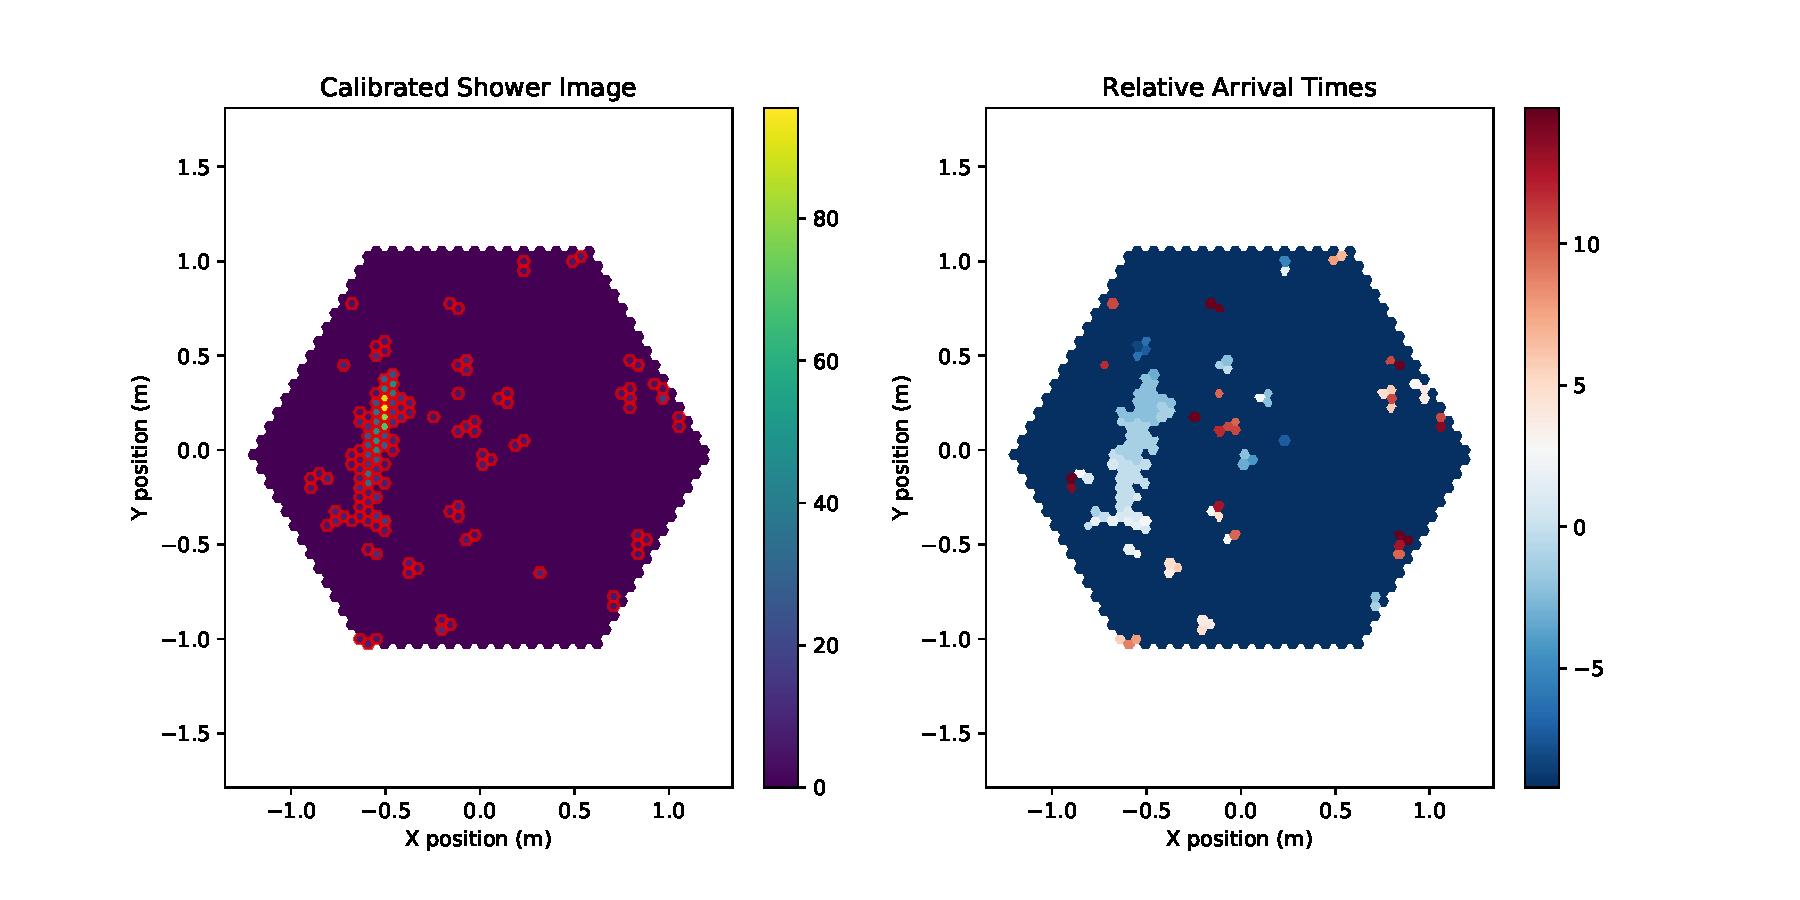
\includegraphics[width=\linewidth]{images/cleaning_plots/fact_2.pdf}
%     \end{figure}
% \end{frame}

% \begin{frame}{Cleaning: FACT approach}
%     \begin{figure}
%         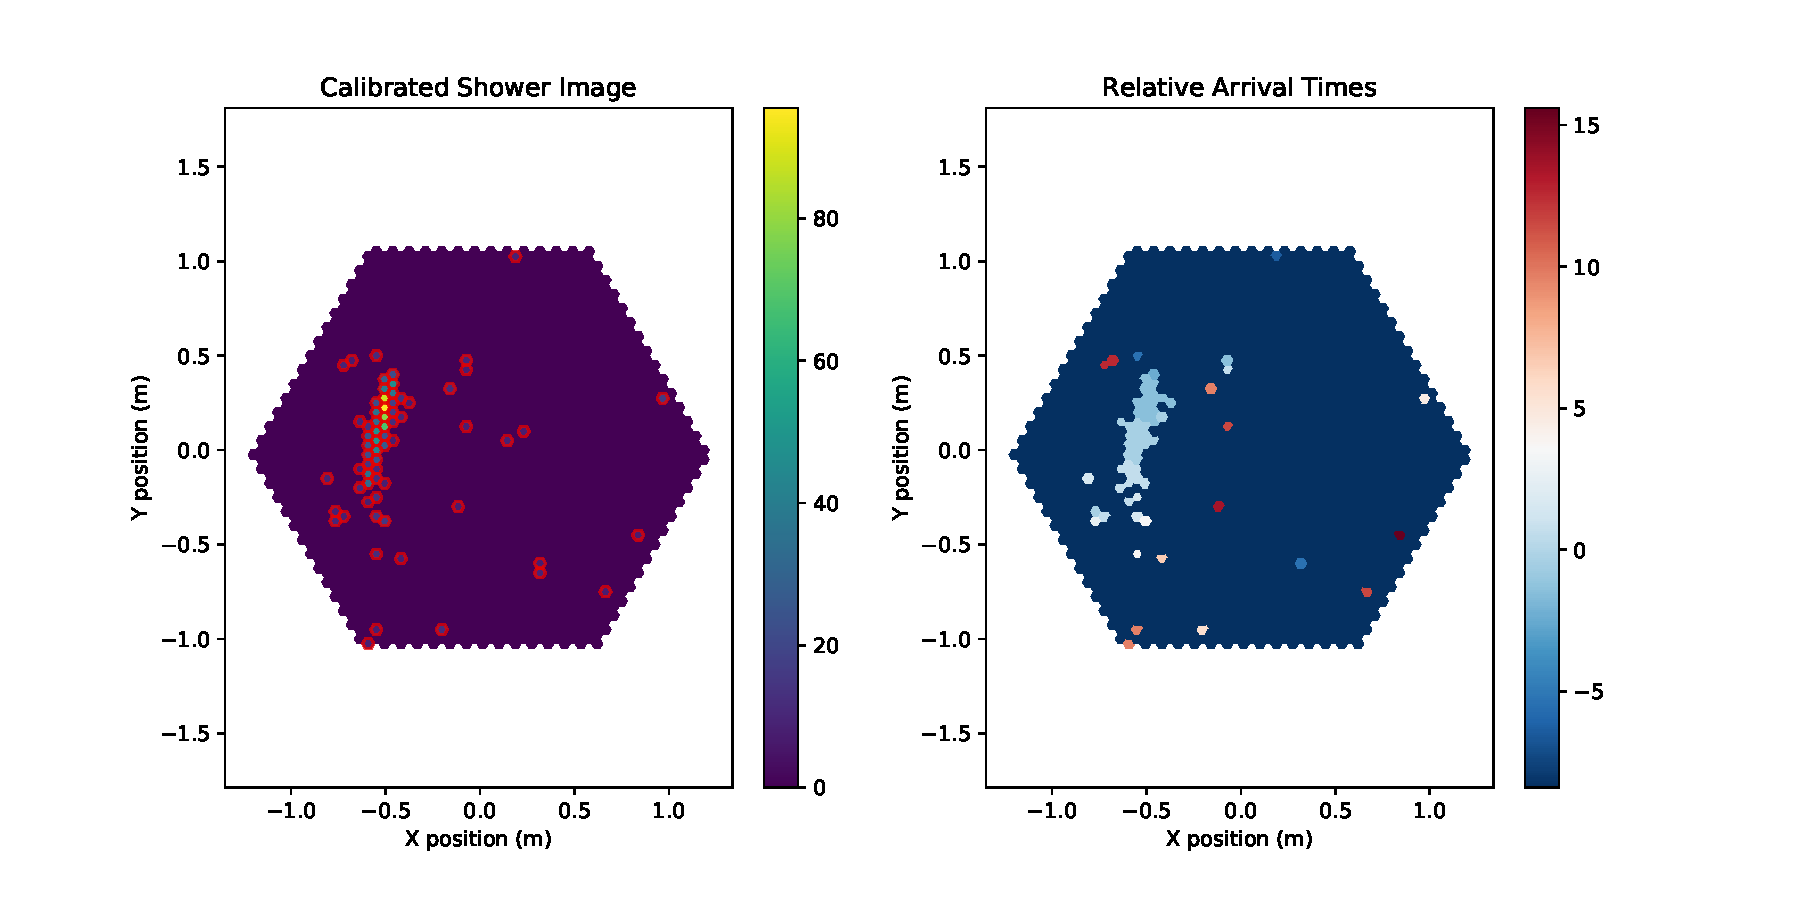
\includegraphics[width=\linewidth]{images/cleaning_plots/fact_3.pdf}
%     \end{figure}
% \end{frame}

% \begin{frame}{Cleaning: FACT approach}
%     \begin{figure}
%         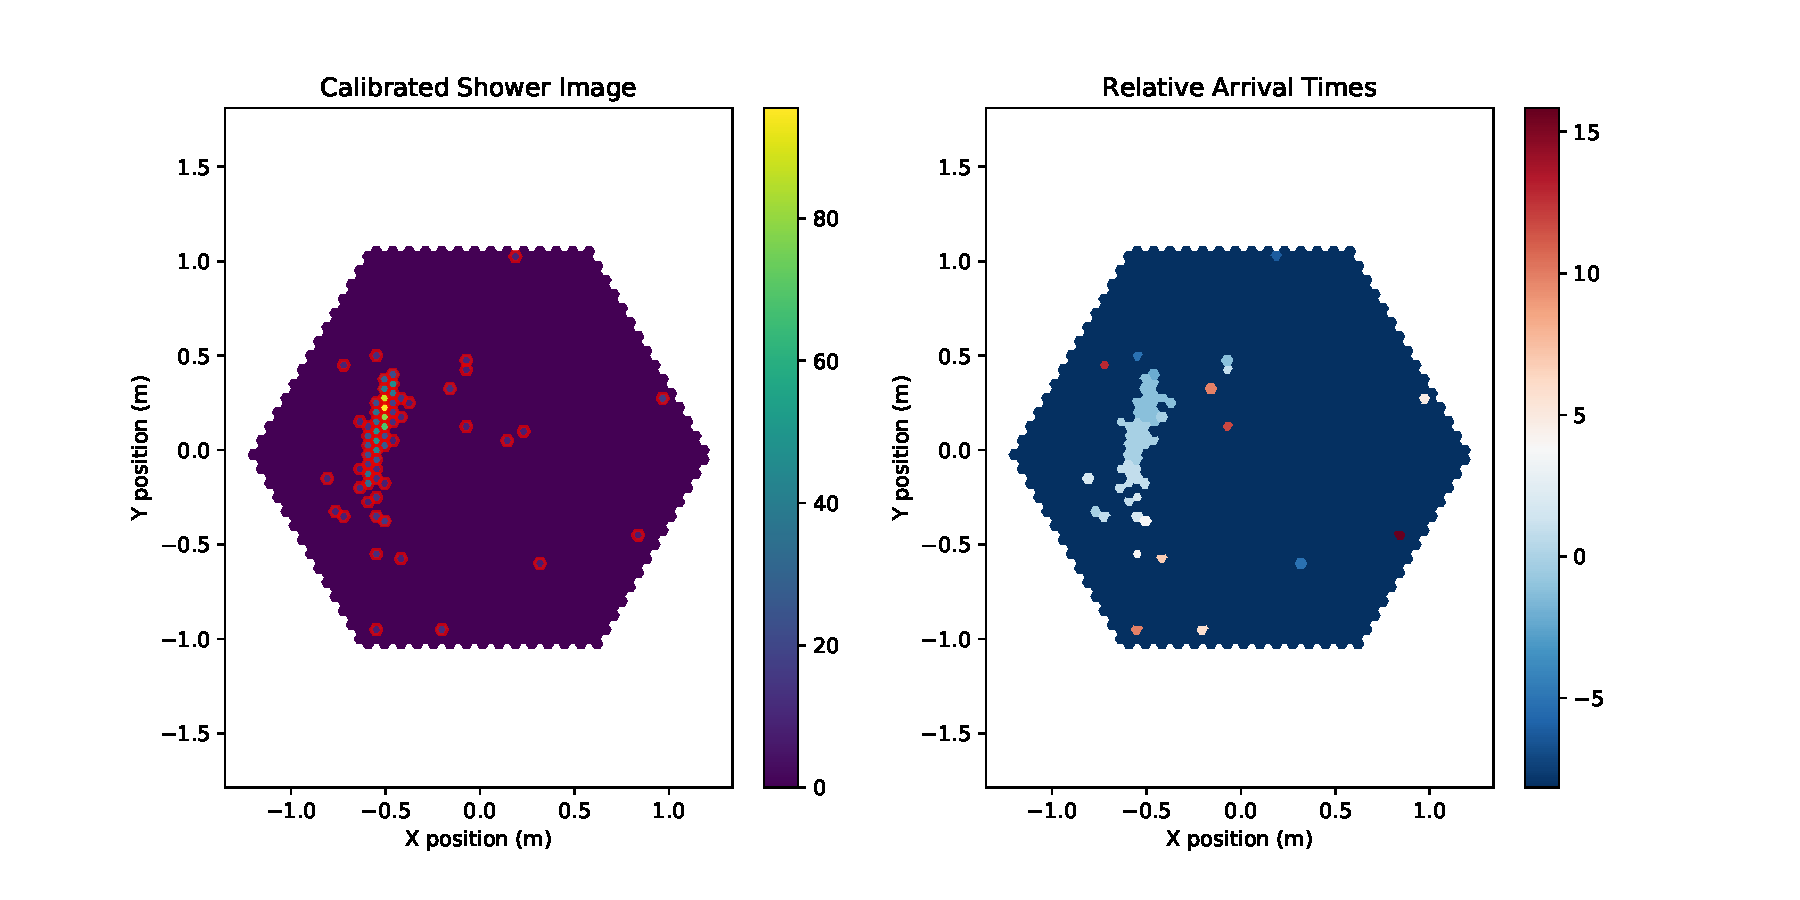
\includegraphics[width=\linewidth]{images/cleaning_plots/fact_4.pdf}
%     \end{figure}
% \end{frame}

% \begin{frame}{Cleaning: FACT approach}
%     \begin{figure}
%         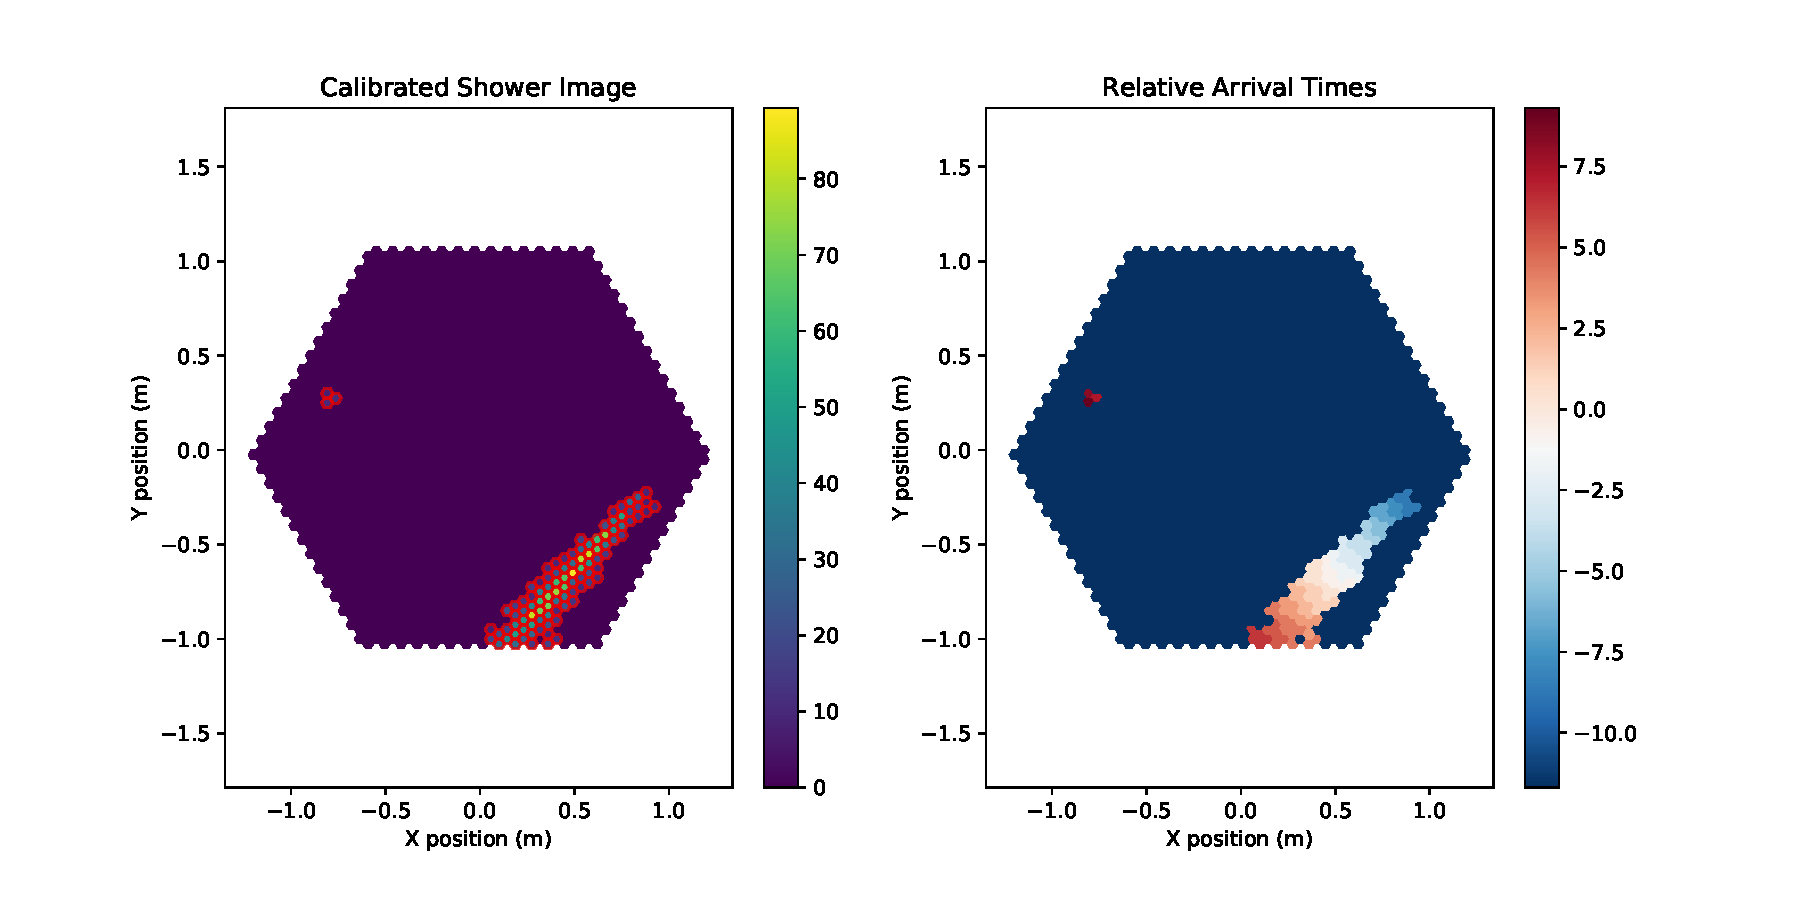
\includegraphics[width=\linewidth]{images/cleaning_plots/fact_5.pdf}
%     \end{figure}
% \end{frame}

% \begin{frame}{Cleaning: FACT approach}
%     \begin{figure}
%         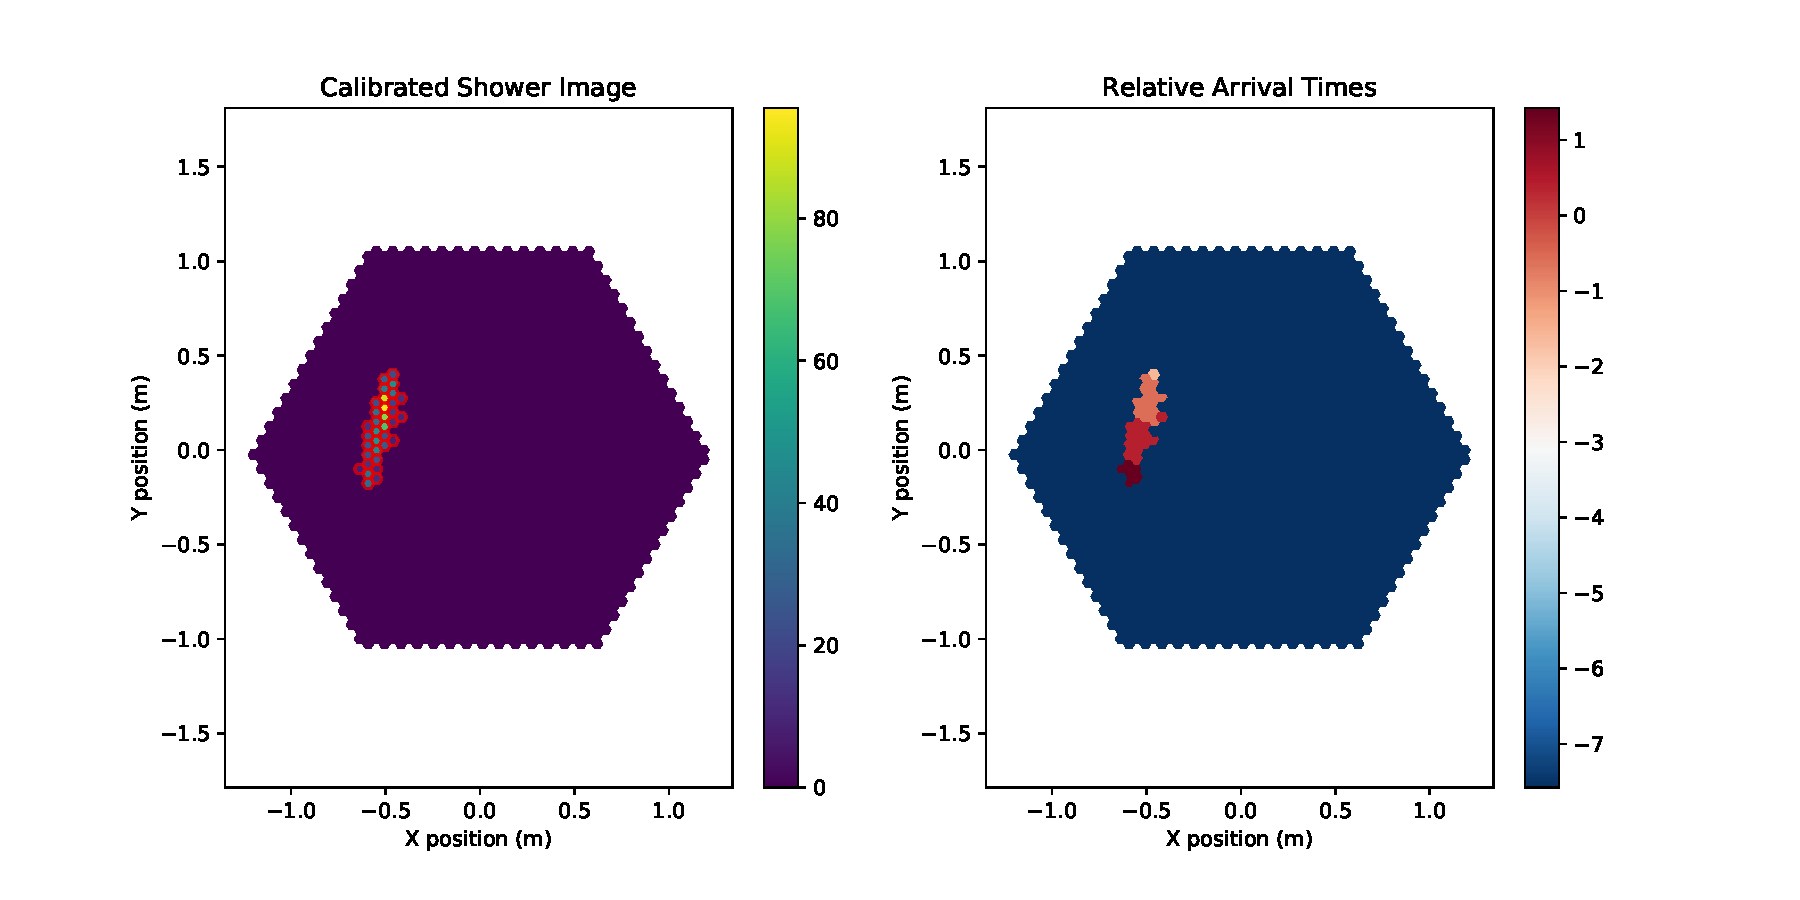
\includegraphics[width=\linewidth]{images/cleaning_plots/fact_6.pdf}
%     \end{figure}
% \end{frame}

\begin{frame}{Comparing the cleaning results}
    \begin{figure}
        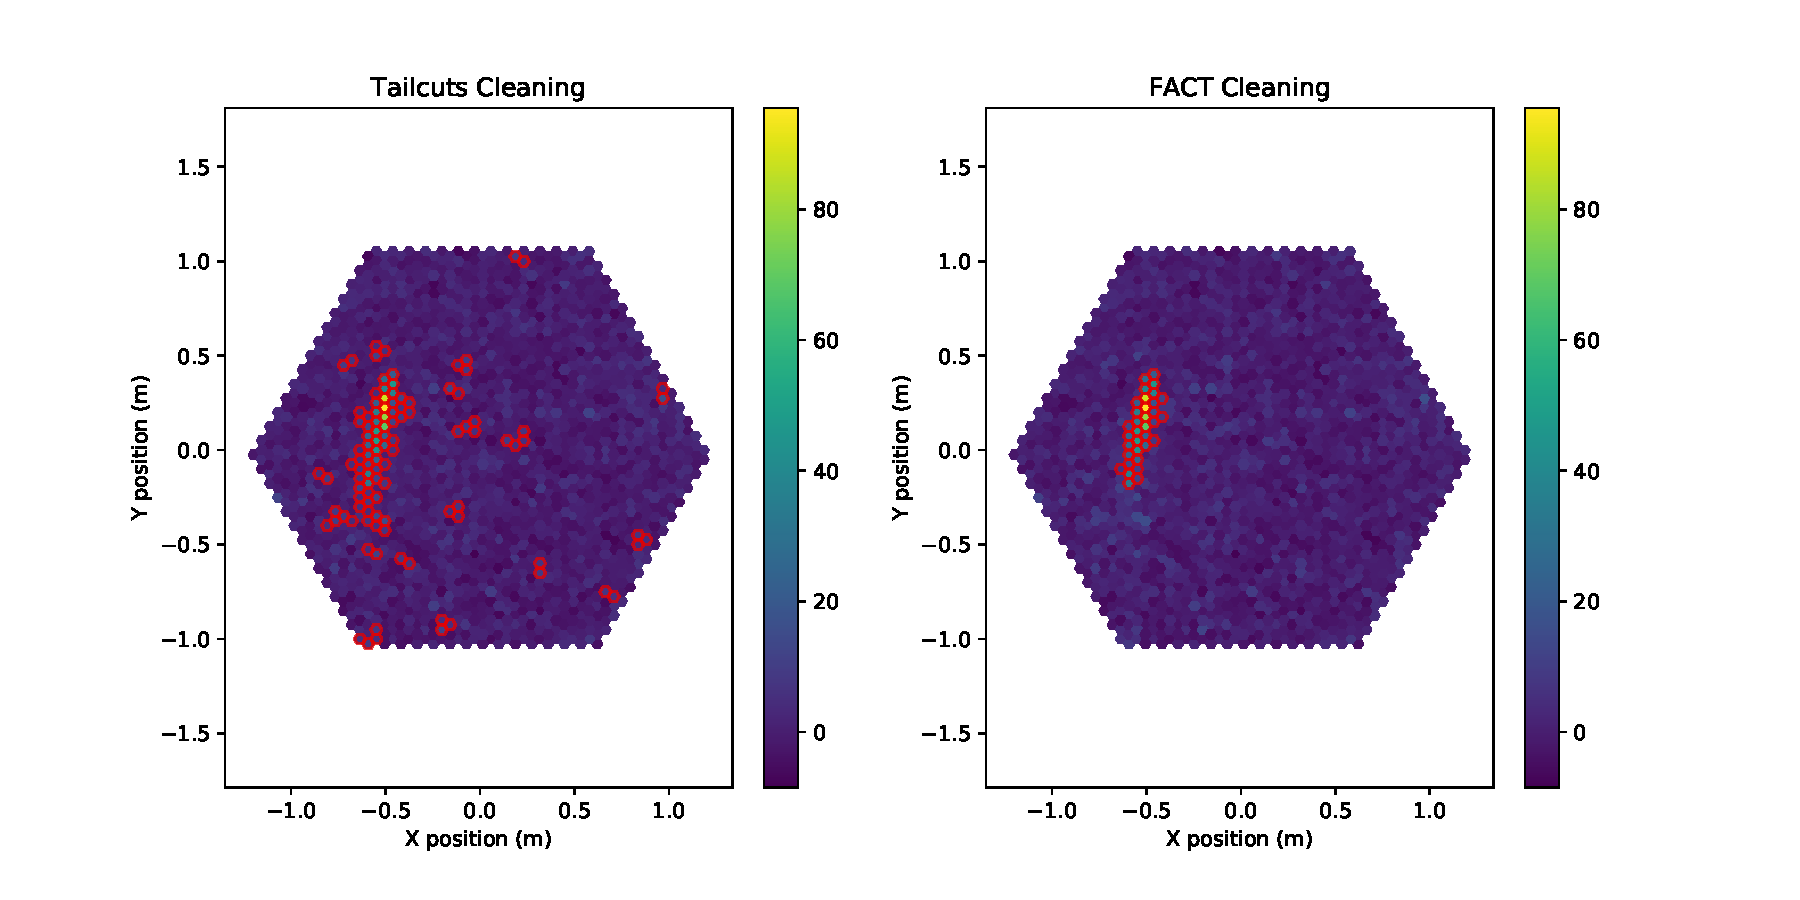
\includegraphics[width=\linewidth]{images/cleaning_plots/comparison.pdf}
    \end{figure}
    % \rightarrow The FACT approach cleans harder, removing most of the background.
    % In this case with very supoptimal thresholds the FACT result is 
    % probably superior.
\end{frame}